\chapter{Introdução a biologia molecular do funcionamento gênico}

Biologia molecular estuda a natureza química dos genes. Como a informação genética é codificada, replicada e expressa. Isto inclui os processos celular da transcrição, tradução e regulação do gene \cite{Pierce2012}. Neste capitulo será revisado os processos dentro da biologia molecular, com ênfase na regulação de um gene no nível transcricional.

\section{Ácidos nucleicos}\label{acidos}

Existe uma grande diversidade de seres vivos, mas a codificação das instruções de todos os organismos vivos estão escritas na mesma linguagem, a "linguagem" dos ácidos nucleicos. Estas são moléculas que exercem um importante papel nos organismos vivos, porque nelas, estão contidos o material genético. Um grande número de informação esta armazenado no material genético, instruções de todas as peculiaridades e funções dos organismos. É a partir do material genético que as células recebem instruções de quais proteínas sintetizar e em que quantidade. Essa informação é decifrada através do código genético, cuja a tradução resulta na síntese de proteínas \cite{Zaha2000}. Existem dois tipos de ácidos nucleicos: ácido desoxirribonucleico (DNA) e ácido ribonucleico (RNA), ambos os ácidos são compostos por nucleotídeos. Os nucleotídeos são formados a partir de três componentes químicos: um açúcar, uma base nitrogenada e um ácido fosfórico (Figura \ref{fig:nucleotideo}). Os nucleotídeos estão ligados entre eles formando uma sequência linear (Figura \ref{fig:sequencia_nucleotideo}).

\begin{figure}[htb!]
    \centering
    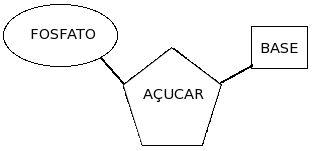
\includegraphics[scale=0.7]{./figuras/componentes_nucleotideo.png}
    \caption{Componentes de um nucleotídeo}
    \label{fig:nucleotideo}
\end{figure}

\begin{figure}[htb!]
    \centering
    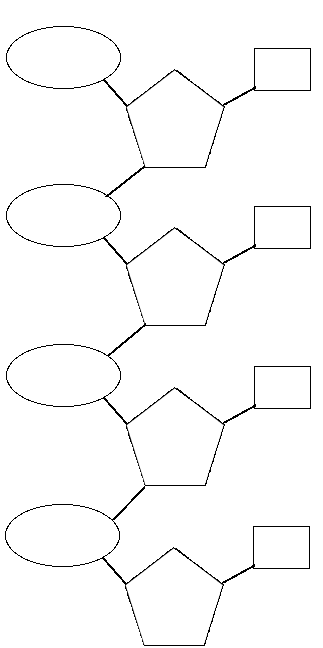
\includegraphics[scale=0.5]{./figuras/sequencia_nucleotideo.png}
    \caption{Sequência linear de nucleotídeos ligados}
    \label{fig:sequencia_nucleotideo}
\end{figure}

Existem duas importantes diferenças entre o RNA e o DNA, que são: o tipo de açúcar e as bases nitrogenadas. O açúcar no DNA é a desoxirribose e no RNA a ribose (Figura \ref{fig:tipos_acucar}). Em cada ácido nucleico são encontradas quatros bases nitrogenadas, sendo que três delas são compartilhadas entre o RNA e DNA são elas: adenina (A), guanina (G) e citosina (C). A base timina (T), é encontrada só no DNA, e a uracila (U), é encontrada só no RNA. Porém existe outra grande diferença entre o RNA e o DNA no nível estrutural. O RNA geralmente existe como uma única sequência de nucleotídeos, enquanto o DNA existe como duas sequências de nucleotídeos pareadas que formam um helicoide, conhecido como dupla hélice. Na Figura \ref{fig:estrutura_DNA_RNA}, podemos observar a estruturas dos dois ácidos. As bases nitrogenadas no DNA estão no interior da hélice, ligadas por pontes de hidrogênio formando pares de bases nitrogenadas (pb). Os únicos pares possíveis no DNA são: A ligado com T e C ligado com G \cite{Zaha2000}.

\begin{figure}[htb!]
    \centering
    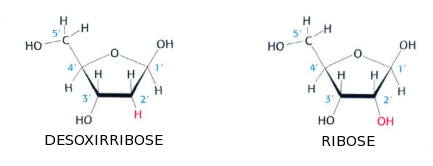
\includegraphics[scale=0.7]{./figuras/tipos_acucar.png}
    \caption{Tipos de açúcar encontrados nos ácidos nucleicos. \cite[Adaptada]{Berg2007})}
    \label{fig:tipos_acucar}
\end{figure}


\begin{figure}[htb!]
    \centering
    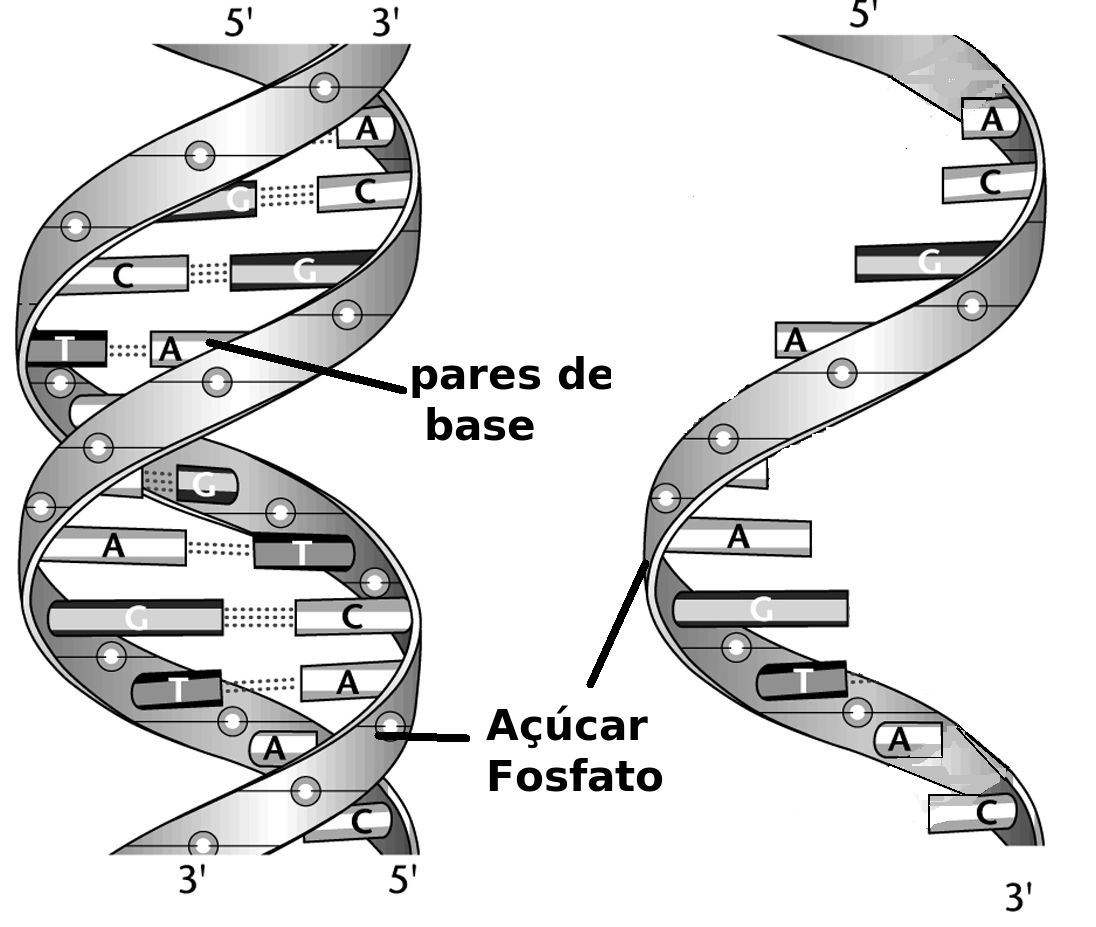
\includegraphics[scale=0.7]{./figuras/estrutura_DNA_RNA.jpg}
    \caption{Estrutura do DNA e RNA. \cite[Adaptada]{Higgs2005}}
    \label{fig:estrutura_DNA_RNA}
\end{figure}

Quanto a estrutura do RNA, ele pode ser dividido em várias classes conforme a sua funcionalidade na célula. A Tabela \ref{T1} mostra as diferentes classes de RNA e suas funcionalidades. 
\begin{table}
\begin{tabularx}{\textwidth}{ |X|X|X|X|X| }    \hline \label{T1}
		  	Classe de RNA      & Função          \\ \hline \hline

    RNA ribossômico (rRNA)  & Componentes estrutural e funcional do ribossomos  \\ \hline
	RNA mensageiro (mRNA)   & Carrega o código genético para a síntese de proteínas\\ \hline
    RNA transportador (tRNA)& Transporta aminoácidos para o mRNA durante a síntese de proteínas \\ \hline
	\textit{Small nuclear RNA} (snRNA)& Processamento do pre-RNA \\ \hline
	\textit{Small nucleolar RNA} (snoRNA)& Processamento e montagem do rRNA \\ \hline
	\textit{Small cytoplasmic RNA} (scRNA)& Variável\\ \hline
	\textit{MicroRNA} (miRNA)& Inibe a tradução do mRNA \\ \hline
	\textit{Small interfering RNA} (siRNA)& Inicia a degradação de outras moléculas de RNA \\ \hline
	\textit{Piwi-interacting RNA} (piRNA)& Pouco sabe-se de sua função\\ \hline					

\end{tabularx}
\caption{Funcionalidades das diferentes classes de moléculas de RNA}
\end{table}
O RNA apesar de ter apenas uma cadeia de nucleotídeos também tem bases complementares. Na síntese de RNA, descrita com mais detalhes na Seção \ref{trans}, as bases que compõem a sequência do RNA são o complemento das bases copiadas do filamento (sequência de nucleotídeos) do DNA modelo, com a substituição de T por U no RNA . As bases complementares no RNA são: A ligado com U e C ligado com G. 


A Figura \ref{fig:repre_sequencia}, mostra uma sequência de DNA e uma de RNA. Elas são comumente representas como uma palavra formada pelo alfabeto (A, G, C, T), para representações de DNA e (A, G, C, U), para representações do RNA. A leitura é feita da esquerda para a direita, no sentido indicado como 5'$\rightarrow$ 3'. Este tipo de representação torna fácil a visualização, assim como a manipulação a nível computacional, sendo amplamente utilizado em métodos \textit{in silico} que envolvem o DNA e o RNA.

\begin{figure}[htb!]
    \centering
    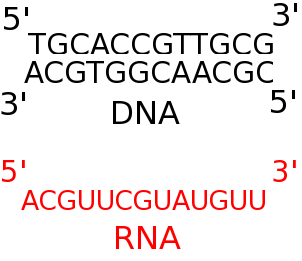
\includegraphics[scale=0.7]{./figuras/repre_sequencia.png}
    \caption{Reapresentação do RNA e DNA}
    \label{fig:repre_sequencia}
\end{figure}

A interação entre o RNA e DNA ocorre quando é necessário a expressão de um gene. Uns dos primeiros passos para a expressão genética é um processo chamado transcrição (Seção \ref{trans}). Neste processo ocorre a formação do RNA (síntese de RNA), a partir de um dos filamentos do DNA. A sequência de RNA formada é uma cópia exata de uma região do RNA. Uma parte desta região que é copiada pertence a um gene. Os genes são seguimentos de DNA podendo ter milhares de pares de bases. São eles que irão especificar o tipo de proteína a ser sintetizado. O processo da síntese de proteínas é conhecido como tradução (Seção \ref{traducao}). A Figura \ref{fig:passo_expresscao_genica}, apresenta cada passo deste conjunto de processos, que também é comumente conhecido como o dogma central.
% talvez falar sobre a importancia da expressão genica

\begin{figure}[htb!]
    \centering
    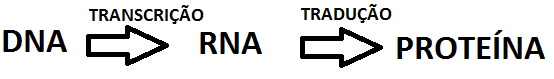
\includegraphics[scale=0.7]{./figuras/passo_expresscao_genica.png}
    \caption{Principais passos da expressão de genética}
    \label{fig:passo_expresscao_genica}
\end{figure}

\section{Proteínas}

Proteínas são os componentes principais de todos os seres vivos. Muitas proteínas são enzimas, que atuam como catalizadores biológicos em reações químicas na célula. Outras são componentes estruturais na célula, provendo suporte para membranas, filamentos, ossos, e cabelo. Algumas proteínas ajudam no transporte de substancias, e outras tem funções regulatórias, de comunicação ou de defesa \cite{Pierce2012}.

As proteínas são compostas por uma sequência de aminoácidos. No total são encontrados pelo menos vinte aminoácidos nas proteínas.

Assim como os ácidos nucleicos a estrutura molecular das proteínas tem vários níveis de organização. A primeira estrutura da proteína é a sequência de aminoácidos. A segunda estrutura deriva da interação entre os aminoácidos que faz a estrutura dobrar-se, semelhante ao helicoide do DNA. A terceira estrutura é a forma tridimensional formada pela ligação dos aminácidos na primeira estrutura. A quarta estrutura é a ligação de várias cadeias polipeptídicas\footnote{Cadeias polipeptídicas são cadeias formadas por mais de vinte aminoácidos}. A Figura \ref{fig:estrutura_Proteinas} apresenta as quatro estruturas das proteínas.

\begin{figure}[H]
    \centering
    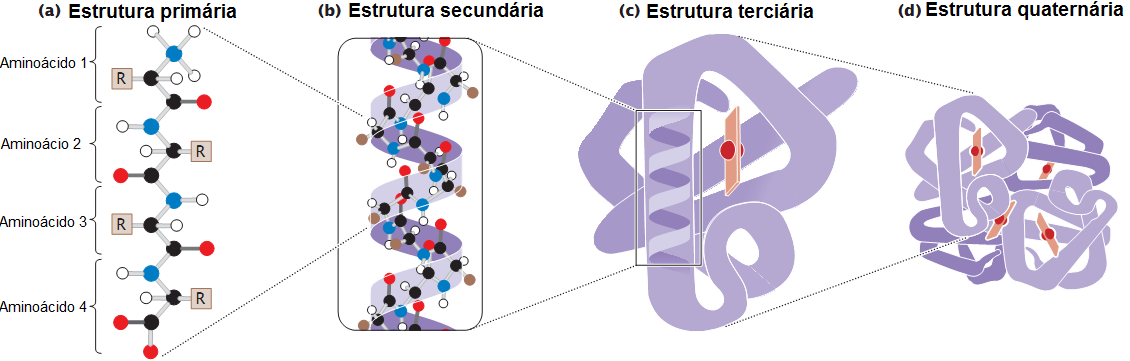
\includegraphics[scale=0.5]{./figuras/estrutura_Proteinas.png}
    \caption{As quatro estruturas das proteínas: (a) A primeira estrutura de uma proteína é sua sequência de aminoácidos; (b) Interações entre aminoácidos faz com que a primeira estrutura se dobre; (c) A segunda estrutura se dobra ainda mais levando a terceira estrutura; (d) Dois ou mais cadeias polipeptídicas associam-se criando a quarta estrutura \cite[Adaptada]{Pierce2012}}
    \label{fig:estrutura_Proteinas}
\end{figure}

\section{Transcrição}\label{trans}

Transcrição é a síntese da molécula de RNA a partir de um molde de DNA. Neste processo uma pequena parte do DNA é copiado. Este tamanho pode variar entre poucos milhares de nucleotídeos, que em comparação com o DNA é muito pequeno, por exemplo uma molécula de DNA no cromossomo humano pode ser maior que 250 milhões de pares de nucleotídeos. Não são todos os genes em uma célula que são transcritos. Porque não é necessário que todas as instruções de funcionamento do organismo seja executada ao mesmo tempo ou na mesma célula \cite{Pierce2012}. A transcrição é um processo altamente seletivo, uma vez que, os genes são transcritos somente quando seus produtos (proteínas) são necessários. Esta seletividade levanta um problema: como reconhecer os genes e transcrevê-los no tempo e local apropriado. 

Para que ocorra a transcrição o primeiro passo é a abertura da hélice dupla do DNA, um dos filamentos do DNA servirá como modelo para a síntese de RNA. A sequência de nucleotídeos na cadeia de RNA é determinada pelo complemento do molde do filamento de DNA (Figura \ref{fig:seq_DNA_molde_e_nao_model}). Qual filamento servirá com molde isso depende do gene que será transcrito. O trecho do DNA que codifica a molécula de RNA e as sequências necessárias para sua transcrição, é chamado de unidade de transcrição. Um complexo de enzimas e proteínas, chamado de aparato de transcrição, reconhece uma unidade de transcrição. Aparece novamente o problema do paragrafo anterior, qual trecho de DNA será lido e como saber o início e a fim dessa leitura. Todas essas informações estão incluídas na sequência do DNA \cite{Pierce2012}. 

Dentro da unidade de transcrição há três regiões: um promotor, uma sequência de codificação do RNA, e um finalizador (Figura \ref{fig:unidade_de_transcricao}). O promotor é uma sequência que o aparato de transcrição reconhece e liga-se. Ele indica qual filamento de DNA será transcrito, em qual direção, e qual é o sítio de início da transcrição (TSS, do inglês \textit{transcription start site}). O TSS é o local onde inicia-se a transcrição, ou seja o primeiro nucleotídeo a ser transcrito. A localização do promotor na unidade de transcrição é antes do TSS e ele não é transcrito em RNA. A segunda região na unidade de transcrição é a sequência de codificação do RNA, a sequência de nucleotídeos de DNA nessa região é transcrita para RNA. A terceira região é o finalizador, uma sequência de nucleotídeos que sinaliza onde é o fim da transcrição. Os finalizadores também fazem parte do RNA, a transcrição para após o finalizador ser copiado \cite{Pierce2012}. Uma definição quanto a direção da transcrição e localização dos nucleotídeos aparece. A direção que o complexo de transcrição se move é chamada de \textit{downstream}, a direção oposta é chamada de \textit{upstream}. Quanto a localização dos nucleotídeos na sequência de DNA, ocorre da seguinte maneira. O primeiro nucleotídeo a ser transcrito (TSS) é numerado com +1, e todos os nucleotídeos localizados \textit{downstream} do TSS são atribuídos números positivos. Nucleotídeos \textit{upstream} do TSS são atribuídos números negativos. Não existe nucleotídeos numerados com 0.


\begin{figure}[H]
    \centering
    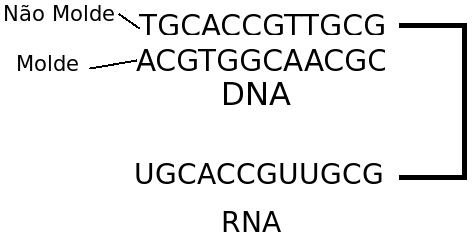
\includegraphics[scale=0.7]{./figuras/seq_DNA_molde_e_nao_model.png}
    \caption{RNA formado, complementar ao filamento modelo}
    \label{fig:seq_DNA_molde_e_nao_model}
\end{figure}

\begin{figure}[H]
    \centering
    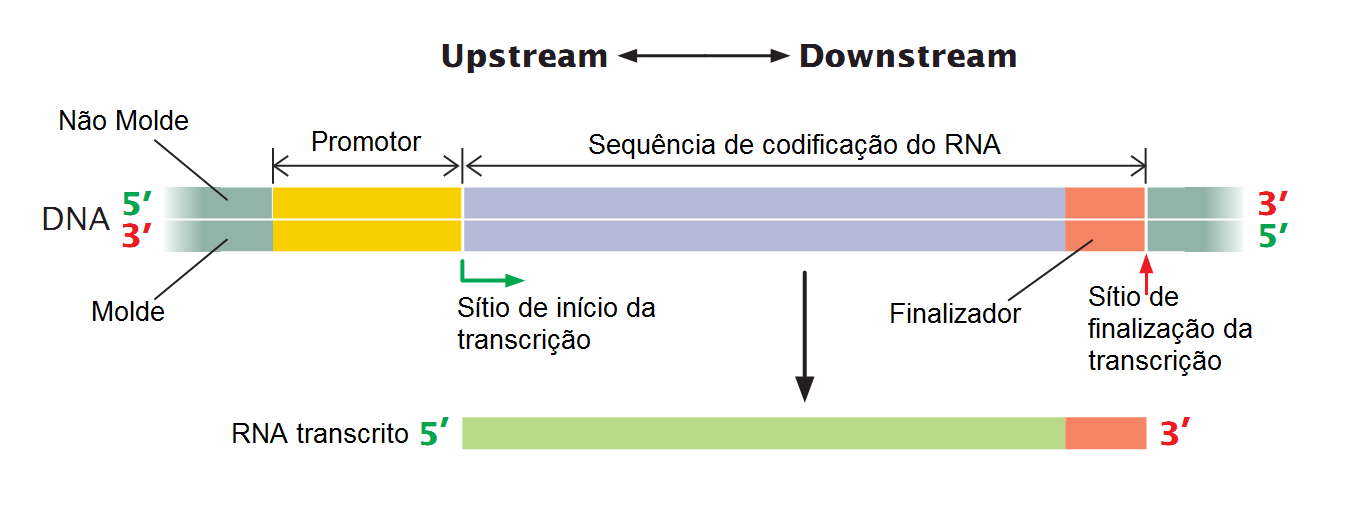
\includegraphics[scale=0.4]{./figuras/unidade_de_transcricao.png}
    \caption{Unidade de transcrição, dividida em promotor, região codificante, e finalizador \cite[Adaptada]{Pierce2012}}
    \label{fig:unidade_de_transcricao}
\end{figure}

Para que ocorra a formação do RNA é necessário a ação de uma enzima que realiza a transcrição, ela é chamada de RNA polimerase. Ela juntamente com proteínas específicas formam o aparato de transcrição. Essas proteínas juntam-se e desconectam-se da RNA polimerase em diferentes níveis no processo de transcrição. Elas atuam como um reforço para a ação da RNA polimerase.

Nos organismos eucarióticos existem três RNA polimerase, chamadas de RNA polimerase I, RNA polimerase II, RNA polimerase III. As três enzimas são similares umas com as outras. A maior diferença entre elas é o tipo de RNA que elas transcrevem:
RNA polimerase I transcreve rRNA; RNA polimerase II transcreve pre-mRNAs, snoRNAs, alguns miRNAs, e alguns snRNAs; e RNA polimerase III transcreve tRNA, pequenos rRNA,alguns miRNAs, e alguns snRNAs (Tabela \ref{TabRNApol}). A RNA polimerase II transcreve a maioria dos genes, ela gera o RNA mensageiro, utilizado na formação das proteínas. 

\begin{table}[H] 
\begin{tabularx}{\textwidth}{ |X|X| }    \hline 
		  	Tipo      & Transcreve\\ \hline \hline

    RNA polimerase I  & grandes rRNAs  \\ \hline
    RNA polimerase II & Pre-mRNA, alguns snRNAs, snoRNAs, alguns miRNAs\\ \hline
    RNA polimerase III & tRNA, pequenos rRNA, snoRNAs, alguns miRNA \\ \hline
\end{tabularx}
\caption{RNA polimerase em eucarióticos \cite[Adaptada]{Pierce2012}}
\label{TabRNApol}
\end{table}

O reconhecimento do promotor é feito por um conjunto de proteínas que ligam-se no promotor para que a RNA polimerase também possa se conectar no promotor. Este conjunto de proteínas pode ser dividido em duas classes. A primeira composta pelos fatores de transcrição gerais, que juntamente com a RNA polimerase formam o aparato basal de transcrição. Este é formado por um grupo de proteínas que se ligam próximo do TSS, ele é suficiente para iniciar a transcrição em seu nível minimo. A outra classe é formada pelos fatores de transcrição específicos que se ligam a específicos segmentos de DNA, aumentando o nível de transcrição pela estimulação do aparato de transcrição na TSS \cite{Pierce2012}. Neste trabalho será apresentado apenas o processo de transcrição com a RNA polimerase II, que transcreve os genes que codificam proteínas. Os promotores encontrados na RNA polimerase II, é dividido em duas partes: promotor principal e promotor regulatório.

O promotor principal está localizado \textit{upstream} do gene e é o local onde o aparato basal de transcrição se conecta. O promotor principal inclui uma ou mais sequências consenso. Por exemplo um sequência consenso comum é a TATA-box, que é formada pela sequência TATAAA e é localizada aproximadamente -25 a -30 pares de base \textit{upstream} do TSS. A Figura \ref{fig:seq_consenso} mostra a TATA-box assim com sequências consensos adicionais.


\begin{figure}[H]
    \centering
    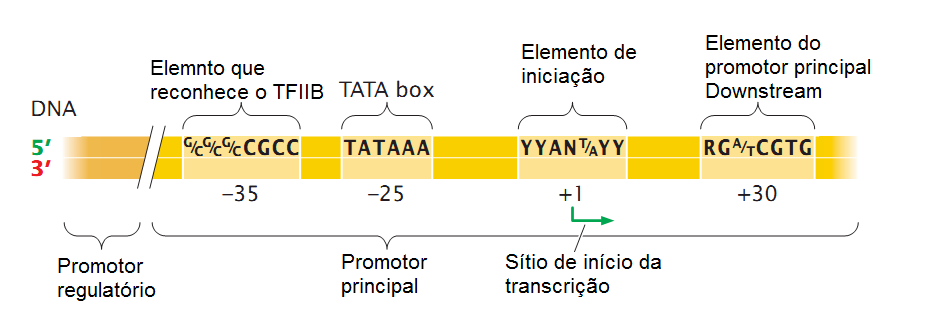
\includegraphics[scale=0.7]{./figuras/seq_consenso.png}
    \caption{Promotor e algumas sequências promotoras, nem todas as sequências mostradas são encontradas em todos os promotores \cite[Adaptada]{Pierce2012}}
    \label{fig:seq_consenso}
\end{figure}

O promotor regulatório é localizado \textit{upstream} do promotor principal. Neste promotor uma variedade de sequências consenso pode ser encontrada. Os fatores de transcrição específicos ligam-se a essas sequências e direto ou indiretamente faz contato com o aparato basal de transcrição, afetando a taxa que a transcrição é iniciada (Figura \ref{fig:promotor_regulacao}). Os fatores de transcrição específicos podem se conectar em sequências distantes chamadas de acentuadores. O DNA entre um acentuador e  promotor forma uma dobra, e os fatores de transcrição ligados no acentuador podem interagir com o aparato de transcrição basal no promotor principal \cite{Simmons2003}.

\begin{figure}[H]
    \centering
    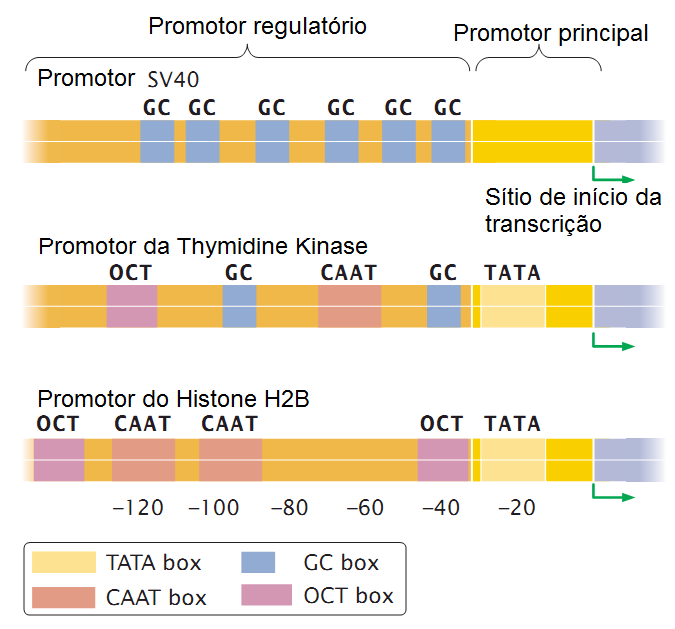
\includegraphics[scale=0.7]{./figuras/promotor_regulacao.png}
    \caption{ Três sequências promotoras de diferentes genes, note como as sequências consenso são ordenadas em diferentes combinações em cada gene\cite[Adaptada]{Pierce2012}}
    \label{fig:promotor_regulacao}
\end{figure}

Os fatores de transcrição gerais que formam o aparato basal de transcrição são: TFIIA, TFIIB, TFIID, TFIIE, TFIIF e TFIIH, onde TF é a sigla para \textit{trancription factor} em inglês, a numeração II indica a RNA polimerase II e a letra identifica um fator de transcrição individual. O complexo formado é apresentado na Figura \ref{fig:iniciacao_trans}. 


\begin{figure}[H]
    \centering
    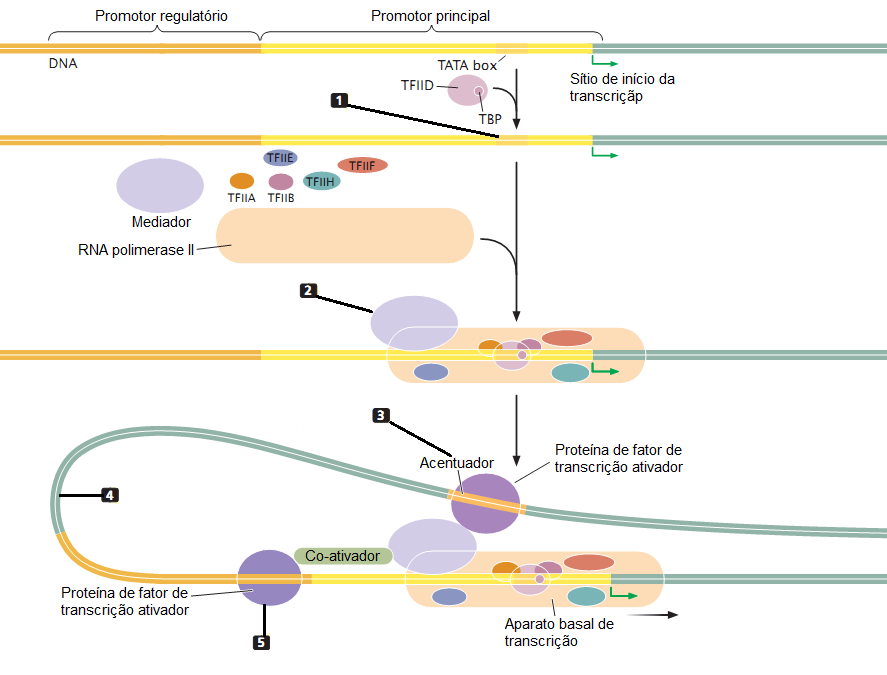
\includegraphics[scale=0.7]{./figuras/iniciacao_trans.png}
    \caption{ Início da transcrição com a RNA polimerase II: (1) TFIID conecta-se na TATA-box no promotor principal; (2) Fatores de transcrição e a RNA polimerase II conectam-se no promotor principal; (3) Proteínas de fator de transcrição específico conectam-se em sequências acentuadoras; (4) DNA faz uma volta, permitindo que proteínas se conectem nos acentuadores para interagir com o aparato basal de transcrição; (5) Proteínas de fatores de transcrição específico conectam-se nas sequências no promotor regulatório e interagem com o aparato basal de transcrição através de um mediador \cite[Adaptada]{Pierce2012}}
    \label{fig:iniciacao_trans}
\end{figure}

O primeiro passo para o inicio da transcrição é o TFIID se conectar na sequência de DNA TATA-box e separar parcialmente os filamentos. Outros fatores de transcrição se conectam em outras sequências consenso no promotor principal, na RNA polimerase e posicionam ela sobre o TSS.

Após a conexão da RNA polimerase e dos fatores de transcrição, formando o aparato de transcrição, a sequência de DNA é separada então a RNA polimerase move-se ao longo do DNA na direção 5' para a 3', deixando o promotor e muitos fatores de transcrição, formando a cadeia de RNA que vai se alongando um nucleotídeo por vez, terminando com uma sequência de nucleotídeos exatamente complementar ao filamento de DNA usado como modelo (Figura \ref{fig:Rnapolimerase}).  Após terminada a cópia a cadeia de RNA, juntamente com a RNA polimerase, se desconectam. A Figura \ref{fig:RNAPOLII} mostra o caminho percorrido da RNA polimerase durante a transcrição.

\begin{figure}[H]
    \centering
    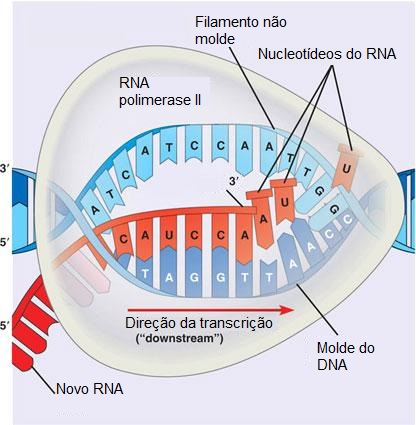
\includegraphics[scale=0.7]{./figuras/RNA-polimerase.jpg}
    \caption{Formação do RNA através da RNA polimerase Fonte: http://www.bio.miami.edu/dana/250/250SS11\_8.html}
    \label{fig:Rnapolimerase}
\end{figure}

\begin{figure}[H]
    \centering
    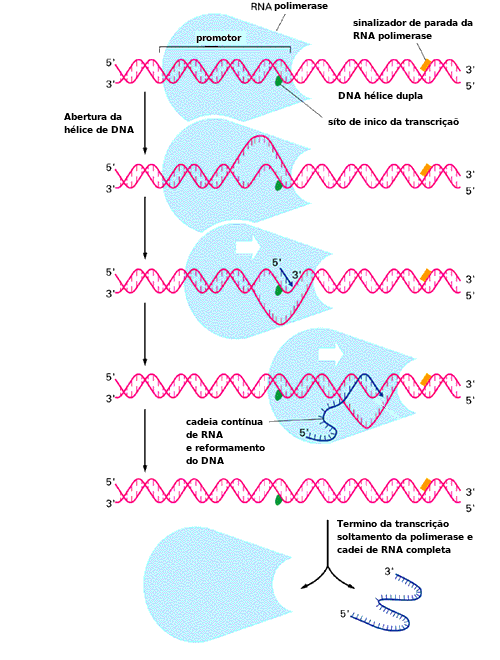
\includegraphics[scale=0.7]{./figuras/RNAPOLII.png}
    \caption{Movimento da RNA polimerase \cite[Adaptada]{Higgs2005}}
    \label{fig:RNAPOLII}
\end{figure}

\section{Código genético}
Como já comentado na Seção \ref{acidos}, a informação codificada no DNA na forma de pares de nucleotídeos é a base para toda a diversidade, funcionalidade, e sobrevivência, nos seres vivos. Para utilizar a informação contida no DNA é necessário decodifica-la. O produto desta decodificação é o código genético.

O código genético é formado a partir da leitura do mRNA, ele é composto por palavras de três nucleotídeos consecutivos. No total são permitidos $4^3 = 64$ possíveis códons \footnote{Códons é a trinca formada pelos nucleotídeos consecutivos}. Sendo que três destes códons são códons finalizadores, especificando o fim da tradução(Seção \ref{traducao}). Os outros 61 códons codificam aminoácidos. Existem vinte aminoácidos mas temos 61 códons para representa-los, isto significa que os aminoácidos são especificado por mais de um códon, com exceção do triptofano e da metionina, que são formados por apenas um códon \cite{Griffiths2000}. Os códons que especificam o mesmo aminoácidos são chamados de sinônimos. A Figura \ref{fig:tab_condos} apresenta os aminoácidos e todos os possíveis códons. Já na Figura \ref{fig:mRNA_to_codon} mostra uma sequência de mRNA decodificada em códons.
 
\begin{figure}[htb!]
    \centering
    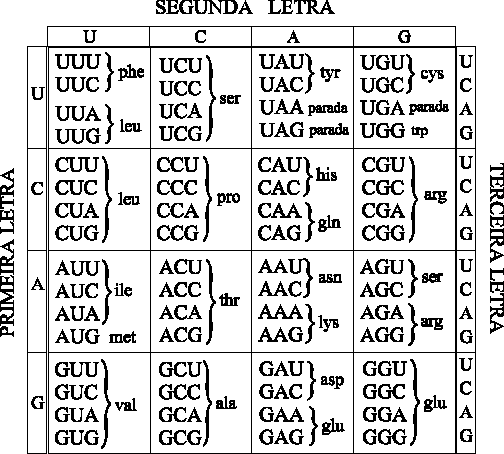
\includegraphics[scale=0.7]{./figuras/tab_condos.png}
    \caption{O código genético formado por 64 códons Fonte: http://www.biomania.com.br/bio/conteudo.asp?cod=1238}
    \label{fig:tab_condos}
\end{figure}

\begin{figure}[htb!]
    \centering
    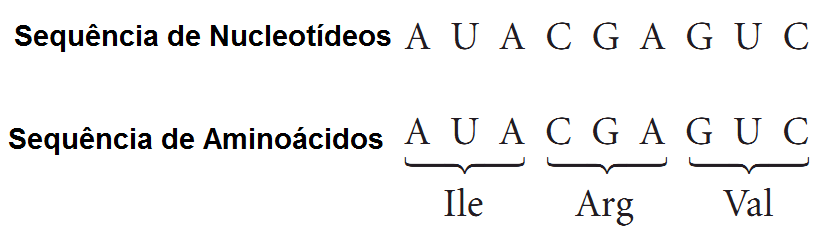
\includegraphics[scale=0.7]{./figuras/mRNA_to_codon.png}
    \caption{Decodificação do mRNA para aminoácidos}
    \label{fig:mRNA_to_codon}
\end{figure}


\section{Tradução} \label{traducao}
A tradução é processo da síntese da proteína a partir do mRNA. Diferente da transcrição a tradução não ocorre núcleo, mas sim no citoplasma da célula onde estão localizados o ribossomos. Os ribossomos são formados de duas subunidades, uma grande e uma pequena. Na tradução mRNA é decodificado para produzir uma sequência de polipeptídeo de acordo com a trinca no código genético. Ou seja utilizando uma cadeia de mRNA será formado a síntese de uma cadeia de aminoácido que por sua vez formará uma proteína \cite{Simmons2003}. O processo da tradução pode ser dividido em quatro partes: 
\begin{enumerate}

\item  \textbf{Ativação}

Um aminoácido é ligado ao complemento de sua trinca no tRNA. Quando há uma ligação entre um aminoácido e um tRNA, este é chamado de "carregado".
\item \textbf{Iniciação}

Nesta etapa os componentes necessários para a tradução são montados no ribossomo, com a ajuda dos fatores de iniciação, que são proteínas que auxiliam o processo.

\item \textbf{Alongamento}

Nesta fase aminoácidos são juntados um por vez. Os tRNA carregados se conetam formando uma sequência de aminoácidos (cadeia polipeptídica).

\item \textbf{Término}

O último processo, na qual a síntese de proteína para em um códon finalizador e os componentes da tradução são soltos do ribossomo.
\end{enumerate}
Durante ou depois deste processo a cadeia de polipeptídeo assumi as estruturas secundária, terciária e quaternária da proteína. A figura \ref{fig:sintese_proteina} resume o processo da tradução.

\begin{figure}[H]
    \centering
    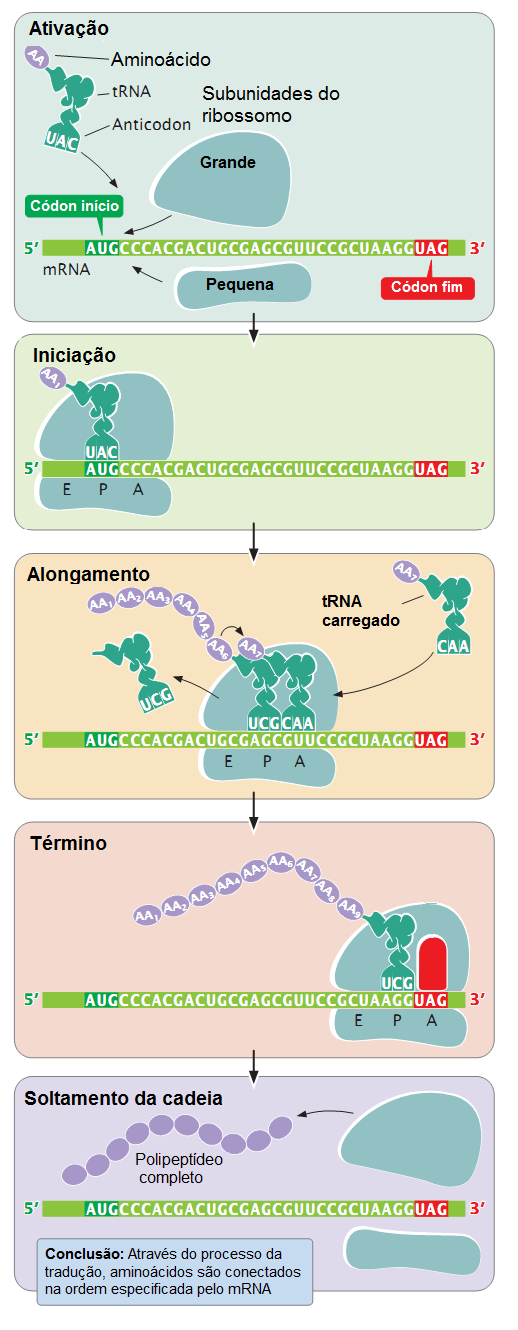
\includegraphics[scale=0.7]{./figuras/sintese_proteina.png}
    \caption{As quatro fases da tradução}
    \label{fig:sintese_proteina}
\end{figure}


\section{Regulação no início da transcrição} \label{S3}

Existem vários níveis de controle da expressão de um gene. Entre estes processão então : a transcrição, alteração da cromatina, alteração da estrutura do DNA, processamento e degradação do RNA, processos que afetam a tradução ou a modificação de proteínas. Nesta seção da continuidade a Seção \ref{trans}, detalhando a ação dos fatores de transcrição específicos, a classificação que os fatores de transcrição recebem segundo suas funções, outras proteínas envolvidas que interagem com eles, e por último genes que têm sua regulação combinada.

Os fatores de transcrição específicos são divididos em duas classes: os ativadores, estimulam a transcrição; e os repressores inibem a transcrição. Os ativadores estimulam e estabilizam o aparato basal de transcrição. Eles podem atuar diretamente com o aparato basal de transcrição ou indiretamente através das proteínas co-ativadoras. Os ativadores podem se conectar em uma sequência de base, geralmente consenso, no promotor regulatório ou em um acentuador. No promotor regulatório há diferentes sequências consenso, em que diferentes fatores ativadores se conectam. Essa sequências consenso são chamadas de elementos regulatórios, e elas podem formar várias combinações (Figura \ref{fig:promotor_regulacao}), então cada promotor é regulado por uma combinação única de fatores de transcrição ativadores \cite{Pierce2012}. Múltiplos elementos de regulatórios formam os CRMs (do inglês, \textit{cis-elements modules}), que integra a conexão de vários fatores de transcrição resultando em um controle combinatório, e em um padrão específico da expressão de um gene \cite{Priest2009}. As funções dos elementos regulatórios e dos CRMs são essenciais as respostas celulares a estímulos \cite{Priest2009}.

A outra classe de fatores de transcrição são os repressores, eles se conectam em elementos regulatórios no promotor regulatório ou em sequências distantes chamadas de silenciadores, que semelhantes aos acentuadores eles são independente de posição e orientação \cite{Pierce2012}. Os repressores competem com os ativadores em três situações:

\begin{enumerate}
\item Se uma região é ocupada por um ativador, a transcrição é ativada, mas se um repressor ocupa o espaço, não há ativação.

\item Um repressor conecta-se próximo a um ativador e impede o ativador interagir com o aparato de transcrição.

\item Um repressor interfere diretamente na montagem do aparato de transcrição, bloqueando a iniciação da transcrição.

\end{enumerate}

\subsection{Regulação combinada}

Alguns genes são ativados pelos mesmos estímulos, eles têm em comum os mesmos elementos regulatórios no promotor ou no acentuador. Estes elementos regulatórios são chamados de elementos de respostas, são sequências pequenas que geralmente têm uma sequência consenso (Tabela \ref{Taq}). Os elementos de resposta são locais de ligação para os fatores de transcrição, que quando ligados aumenta o nível da transcrição. O mesmo elemento de resposta pode estar presente um vários genes permitindo que múltiplos genes sejam ativados pelo mesmo estímulo. Um estímulo pode ser um estresses como mudança na temperatura, mudança hormonal entre outros. Na próxima seção detalharemos um importante fator de transcrição (\textit{dehydration responsive element binding proteins}) que se liga no elemento de resposta \textit{dehydration responsive element}.

\begin{table}[H]
\begin{tabularx}{\textwidth}{ |X|X|X| }    \hline 
		  	Elemento de resposta      & Tipo de resposta & Sequência consenso         \\ \hline \hline

    Heat-shock element & Calor e outros estresses & CNNGAANNTCCNNG \footnote{O \textit{N} no meio da sequência indica que nesta posição pode haver qualquer base} \\ \hline
	Glucocorticoid response element & Glococorticoids & TGGTACAAATGTTCT\\ \hline
    Phorbol ester response element & Phorbal esters & TGACTCA \\ \hline
    Serum response element & Serum & CCATATTAGG \\ \hline
	Dehydration responsive element & mudanças de temperatura, alta salinidade, e seca& A/GCCGAC \footnote{A barra entre as bases A e G, indica que nesta posição pode aparecer tanto A quanto G}\\ \hline

\end{tabularx}
\caption{Alguns elementos de resposta}
\label{Taq}
\end{table}

\section{Dehydration responsive element binding proteins (DREB)}

No amplo conjunto de fatores de transcrição, existem aqueles que quando ligados nos elementos de resposta irão ativar as respostas da célula a estresses abióticos. O estresse abiótico afeta diversos organismos, mas em especial os organismos vegetais que são dependentes de fatores ambientais, são os mais afetados. Nesta seção apresentaremos o \textit{dehydration responsive element binding proteins} (DREB) um importante fator de transcrição nas plantas.

O DREB ativa genes que estão relacionados com a resposta da célula a estímulos abióticos, com a ativação destes genes, a planta se adapta as condições adversas a sua sobrevivência, através de reações bioquímicas e físicas que ocorrem na planta. Os estresses abióticos que mais afetam as plantas são: seca, alta salinidade e mudanças de temperatura. O estresse abiótico atrapalha a sobrevivência e consequentemente a produção de grãos como a soja, arroz, milho e o trigo.

O DREB está contido dentro de uma família de fatores de transcrição única nas plantas, a \textit{Ethylene Responsive Element} (ERF). A ERF desempenha um importante papel em resposta a estímulos abióticos e bióticos. O DREB pode ser dividido em duas subclasses DREB1 e DREB2, envolvidas em estresses de baixa temperaturas e desidratação, respectivamente \cite{Chen2007GmDREB2}.

O elemento de resposta que se conecta no DREB é chamado de \textit{dehydration responsive element} DRE, e ele é formado pela sequência A/GCCGAC \cite{Nakashima2009}. Entretanto para que o DRE seja funcional ele tem que estar acompanhado de elementos regulatórios, mas a especificidade desses elementos regulatórios é baixa, fazendo que muitos desses variem de gene para gene \cite{Zhang2005}. Portanto, em uma busca computacional de genes alvos do DREB (ou outro fator de transcrição), não basta procurar o DRE (ou outro elemento resposta), na região promotora, uma vez que outros elementos regulatórios também participam da regulação, isto torna a busca por genes alvo uma difícil tarefa, uma vez que há uma variação nos elementos regulatórios de um gene para outro.

Segundo \cite{Agarwal2006}, o entendimento do DREB na regulação de um gene é de grande importância para o desenvolvimento de plantas tolerantes a estresses. Já que, estresses abióticos e bióticos influenciam negativamente na sobrevivência e na larga produção de grãos. Culturas como soja, arroz e trigo que são amplamente usadas na alimentação mundial são prejudicadas pelos estresses que muitas vezes impedem uma alta produtividade. 
